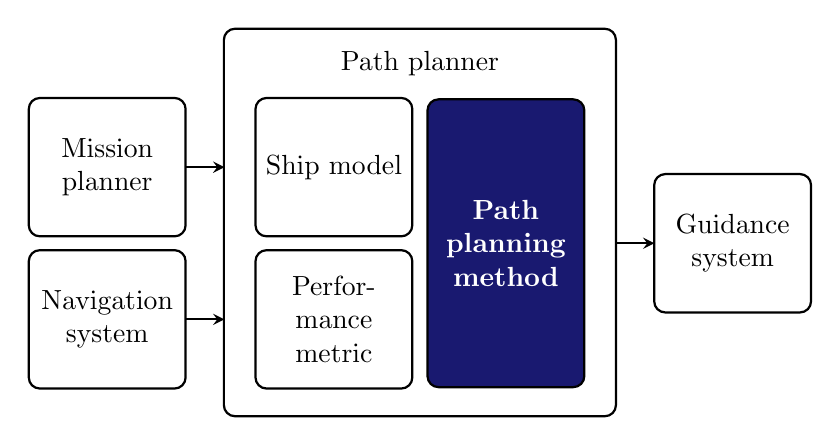
\begin{tikzpicture}[x=5.65em,y=5em]

	\tikzstyle{block} = [rectangle, draw, thick,
    		text width=5em, text centered, rounded corners, minimum height=5em]
	\tikzstyle{block_marked} = [block, fill=MidnightBlue, text=white, font=\bfseries]
	\tikzstyle{plaintext} = [draw=none,fill=none,text width=6em, text centered]
	\tikzstyle{line} = [draw, ->,>=stealth, thick, rounded corners]


    \node [block, text width=13.5em, minimum height=14em] at (0, 0.15) {};
    \node [block_marked, minimum height=10.4em] at (0.55, 0) {Path planning method};
    \node [block] at (-0.55, 0.55) {Ship model};
    \node [block] at (-0.55, -0.55) {Perfor-mance metric};
    
    \node [block] at (-2, 0.55) {Mission planner};
    \node [block] at (2, 0) {Guidance system};
    \node [block] at (-2, -0.55) {Navigation system};
    
    \node [plaintext] at (0, 1.3) {Path planner};
    %\node [plaintext] at (-0.75, 0.75) {Mission};
   % \node [plaintext] at (0.75, 0.75) {Path};
   % \node [plaintext] at (0.5, -0.75) {Navigation Data};
    
    \path [line] (-1.5, 0.55) -- (-1.25, 0.55);
    \path [line] (-1.5, -0.55) -- (-1.25, -0.55);
    \path [line] (1.25,0) -- (1.5, 0);
    
\end{tikzpicture}